\documentclass[final,hyperref={pdfpagelabels=false},xcolor=table]{beamer}
\mode<presentation>{
	\usetheme{ucb}
}
\usepackage[size=custom,width=101.6,height=76.2,scale=1.5]{beamerposter}
\usepackage{multicol}
\usepackage{graphicx}
\usepackage{textcomp}
%\usepackage{booktabs}
%\usepackage{multirow}
%\usepackage{listings}
%\usepackage{siunitx}
\usepackage{blindtext}
\usepackage{pbox}

\graphicspath{{../figures/}}

\definecolor{ucb-pacific}{HTML}{5B6770}

\newcommand{\uT}{{\textmu}T}
\setlength{\leftmargini}{4em}

\title{Nephele: A Simple Solution for Data Replication}
\author{Joao Carreira, Howard Mao, and Nathan Pemberton}
\advisor{Randy Katz}
\institute[UC Berkeley]{\textsc{University of California, Berkeley}}

\begin{document}
\begin{frame}
\vspace{-1.5em}
\begin{columns}[t]
	\begin{column}{0.3\linewidth}
            \begin{block}{Motivation}
    As the number of nodes in distributed systems increases, failures become
    the rule, not the exception. Because of this, it is important to be able to
    recover from crashes quickly and with minimal impact on performance and
    complexity. Checkpointing and manual serialization/deserialization are both
    slow and complicated.
\end{block}

            \vspace{1ex}
            \begin{block}{Architecture}
    \centering
    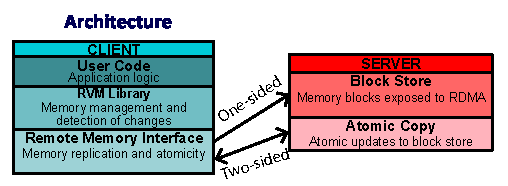
\includegraphics[width=0.9\textwidth]{lasagna.pdf}
\end{block}

            \vspace{1ex}
            \begin{block}{RVM API}
    RVM allows the user to allocate recoverable regions of memory and
    atomically replicate changes to that memory to a remote node’s DRAM. The
    user simply identifies recovery points in their code through a
    transactional API.

    \vspace{1ex}

    \begin{tabular}{ | l | l | }
        \hline rvm\_cfg\_[create/destroy]() & \pbox{20cm}{Initialize the system \\
        and recover memory if needed} \\
        \hline rvm\_[alloc/free]() & \pbox{20cm}{Allocate a region \\
        of recoverable memory} \\
        \hline rvm\_txn\_[start/commit]() & \pbox{20cm}{Mark a point of \\
        consistency in the program} \\
        \hline rvm\_[set/get]\_usr\_data() & \pbox{20cm}{Register a pointer \\
        to your state.} \\
        \hline
    \end{tabular}
\end{block}

            \vspace{1ex}
            \begin{block}{Backends}
    Underneath the RVM layer is a remote memory backend, which handles
    communication with the remote node. The rmem layer implements basic
    functions like \texttt{malloc()}, \texttt{free()}, \texttt{put()},
    \texttt{get()}, and \texttt{commit()}. So far we have implemented two
    different backends. One uses a custom protocol based on Infiniband RDMA.
    The other uses RAMCloud, an Infiniband-based key-value store.
\end{block}

	\end{column}

	\begin{column}{0.3\linewidth}
            We used micro-benchmarks to test the performance of RVM commits and RVM
recovery. To test commits, we allocated a number of pages, made modifications
to each one of them, and measured the time it took for \verb|rvm_txn_commit()|
to complete. To test recovery, we first allocate a number of pages and
close the connection to the server. We then restart the connection using the
recovery flag and time how long it takes \verb|rvm_cfg_create()| to complete.
When benchmarking the IB backend, we run three trials for each number of pages,
restarting the server after each trial.

\subsection{IB Backend}
Figure \ref{fig:ib-commit-ubm} shows the results of the commit micro-benchmark
using the IB backend. At the smallest page count, the commit time is around
150 microseconds. At 10K pages, the commit time has increased to 140 milliseconds.
As can be seen in the graph, the relation between page count and commit time
is fairly linear, with a slope of about 13.7 microseconds per page.

\begin{figure}[h]
    \caption{IB Commit Micro-Benchmark Results}
    \includegraphics[width=\linewidth]{graphs/commit-results-rm.pdf}
    \label{fig:ib-commit-ubm}
\end{figure}

Figure \ref{fig:ib-recovery-ubm} shows the results of the recovery
micro-benchmark using the IB backend. Recovery is quite a bit slower than
commit. Recovering a single page takes about 50 milliseconds, while recovering
10,000 pages takes more than 2 seconds. The relationship between number of
pages and recovery time is also not entirely linear.
The recovery time increases steadily until about 2000 pages, after which it
increases drastically. It is uncertain what is causing this sort of behavior,
as startup time involves a lot of different things, including the allocation
of local memory pages, receiving tag to address mappings from the server, and
copying data from the server.

\begin{figure}[h]
    \caption{IB Recovery Micro-Benchmark Results}
    \includegraphics[width=\linewidth]{graphs/recovery-results-rm.pdf}
    \label{fig:ib-recovery-ubm}
\end{figure}

\subsection{RAMCloud Backend}
\begin{figure}[t!]
\begin{center}
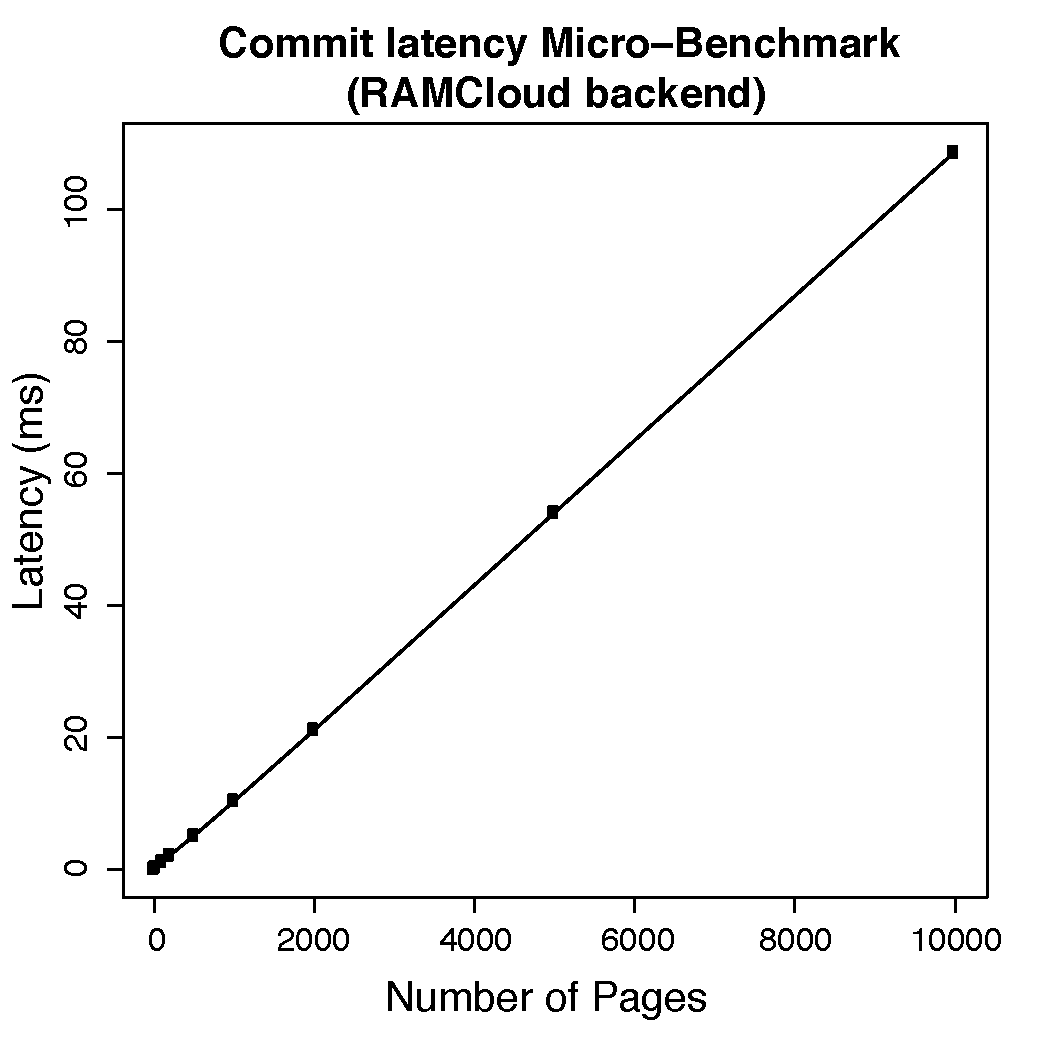
\includegraphics[scale=0.40]{graphs/commit_time_rc_latencies.pdf}
\end{center}
\caption{Commit time micro-benchmark when using the RAMCloud backend}
\label{fig:inmem_fs_design}
\end{figure}

Figure~\ref{fig:inmem_fs_design} shows the results of the commit micro-benchmark when using the RAMCloud backend. 
The end-to-end latency of a commit operation is dominated by the number of pages to be commited, as each page write requires a round-trip to the RAMCloud server.
The RAMCloud backend also needs to save the table that contains the mapping between tags and keys in, but this only requires one interaction with the server.
The RAMCloud backend requires roughly 10 microseconds to write a page to RAMCloud. As can be seen in the graph, the commit time grows linearly with the number of pages as expected.






	\end{column}

	\begin{column}{0.3\linewidth}
            \begin{block}{Macro-Benchmarks}
    \begin{itemize}
        \item \textbf{DGEMV} - Multiply a matrix by a vector and repeat using
            the result. We run using a 100,000 x 100 matrix over 1000
            iterations.  We measure how the total runtime is affected by
            failure rate (the number iterations between restarts) and commit
            rate (number of iterations between commits) and compare the
            results to simply saving the data to a file.
        \item \textbf{Gene Assembly} - Assemble gene sequences from a set of
            k-mers (fixed size gene sequences). We measure how the total
            runtime is affected by commit rate and compare the results to
            process state checkpointing using BLCR.
    \end{itemize}

    \centering

    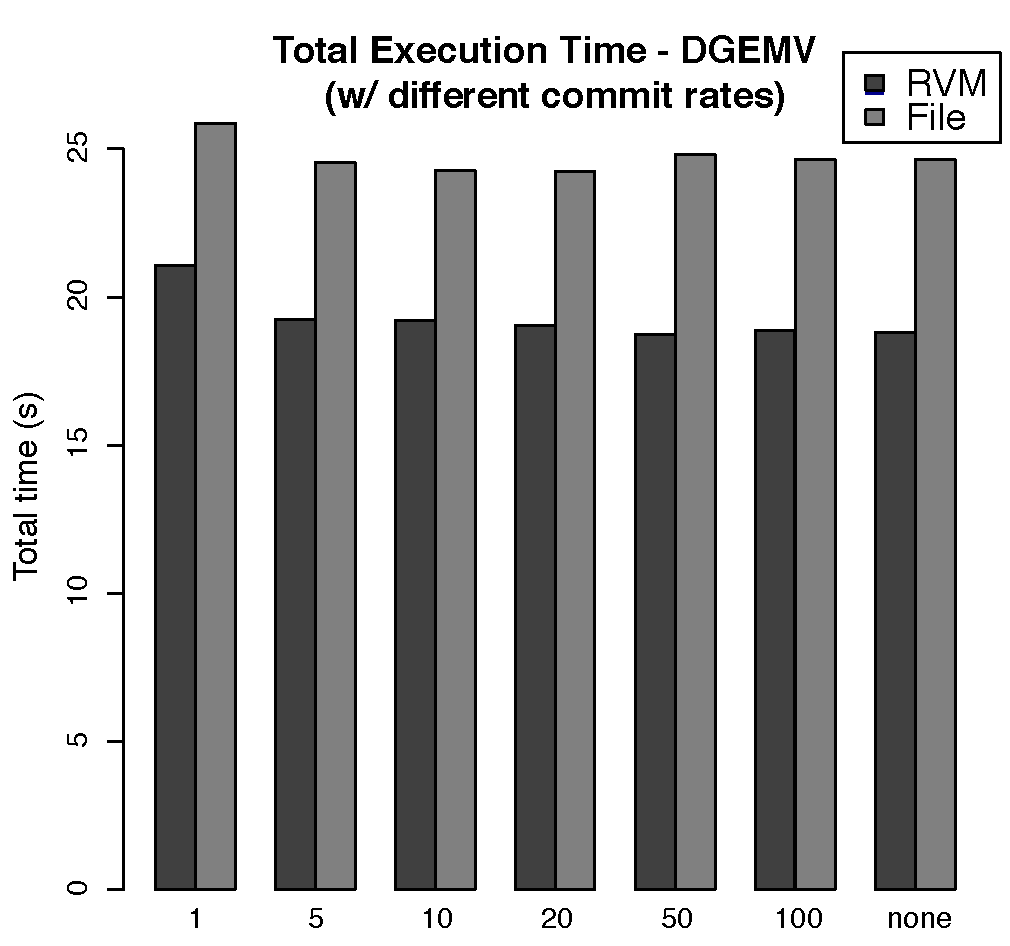
\includegraphics[width=0.45\textwidth]{dgemv_total_time_commit.pdf}
    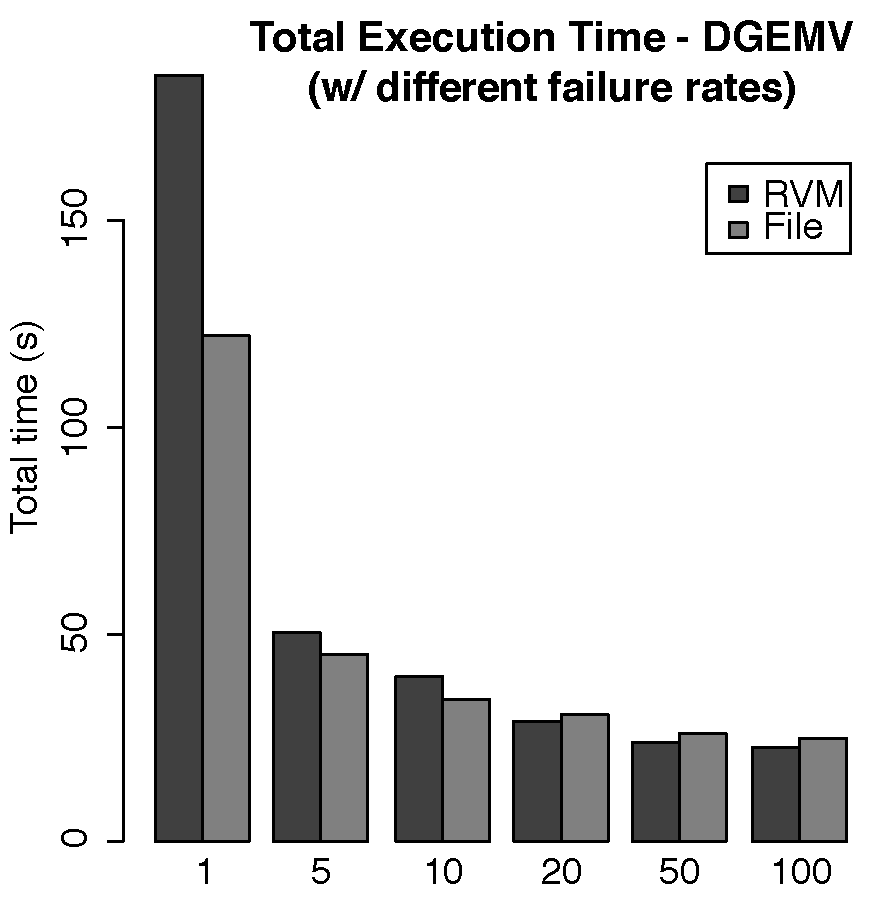
\includegraphics[width=0.45\textwidth]{dgemv_total_time_fail.pdf}

    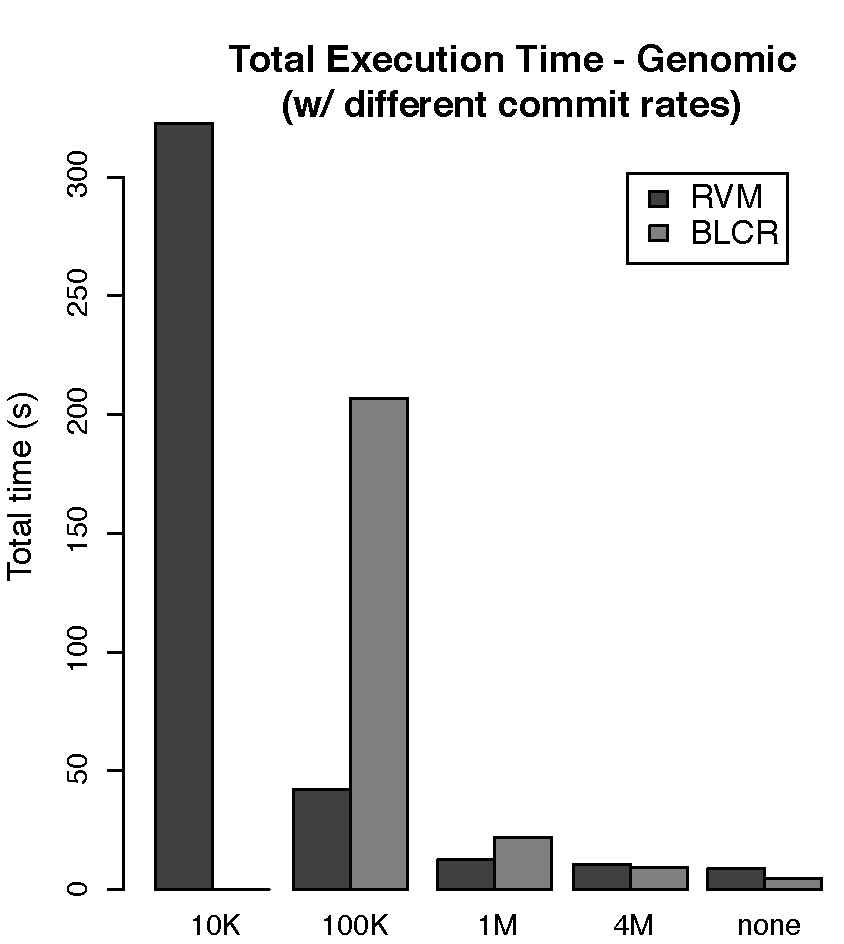
\includegraphics[width=0.45\textwidth]{genome_total_time_commit.pdf}
\end{block}

            \vspace{1ex}
            In this paper, we presented Recoverable Virtual Memory, our solution for easy
replication and recovery of application state. We have attempted to provide our
implementation with features we believe are highly desirable for the
application programmer, such as a simple and understandable API; restoration of
virtual address locations, which allows for recovery of complex data structures
without the need for serialization; and reasonably low overhead.  Of these
three goals, we have accomplished the first two, but there is still
considerable work to be done in regards to performance.

The most obvious optimization we could make is to coalesce RDMA operations for
contiguous pages. In our current infiniband backend, allocation of the backing
memory for multiple contiguous pages must be done a page at a time.  However,
it would be much more efficient to perform a single contiguous allocation on
the server side. That way, the number of RDMA write calls and TXN\_MULTI\_CP
messages does not need to increase as the number of pages increases. There are
probably other areas for performance improvement that we could discover through
more intensive profiling of the benchmark programs.

Another avenue we could explore are alternative backends for the RMEM layer.
There are various networking and non-volatile memory technologies that we could
investigate, such as SSDs and RDMA over Converged Ethernet. We could also
implement different consistency semantics to explore the tradeoffs of
performance and consistency.

Finally, we would like to integrate RVM with existing runtimes and recovery
frameworks to provide a more complete data replication and recovery solution.

The complete code for our RVM implementation is available on GitHub at
https://github.com/zhemao/rmem-server.

	\end{column}
\end{columns}
\end{frame}
\end{document}
